\documentclass[10pt,a4paper]{article}
\usepackage[utf8]{inputenc}
\usepackage[T1]{fontenc}
\usepackage{lmodern}
\usepackage[margin=1.8cm]{geometry}
\usepackage{amsmath,amssymb,amsfonts}
\usepackage{booktabs}
\usepackage{graphicx}
\usepackage{hyperref}
\usepackage{xcolor}
\usepackage{caption}
\usepackage{enumitem}

\hypersetup{
    colorlinks=true,
    linkcolor=blue!60!black,
    citecolor=blue!60!black,
    urlcolor=blue!60!black
}

\title{\textbf{Safe and Smooth Automatic Train Speed Control:\\
From Emulated-Trajectory Shielding to Generalized Multi-Station\\
Hierarchical Contract-Based PPO}}
\author{Technical Project Report}
\date{November 8, 2026}

\begin{document}
\maketitle

\begin{abstract}
Modern railway control is split into two worlds: \textbf{Automatic Train Protection (ATP)}, which enforces strict speed limits using worst-case braking rules (often causing harsh braking and rough rides), and \textbf{Automatic Train Operation (ATO)}, which drives the train smoothly and stops accurately at station platforms, but lacks formal safety guarantees. In this project, we bridge both objectives across a three-stage architectural evolution. In \textbf{Stage 1}, we upgrade an Intelligent-PID (IPID) switcher and a State-Augmented Linear Time-Varying Model Predictive Controller (LTV-MPC), combine them via Reinforcement Learning (RL) trained on a \textbf{Heteroscedastic Neural Physics Emulator}, and wrap the system inside a runtime \textbf{Safety Filter Shield}, achieving $3\text{ mm/s}$ ($0.0030\text{ m/s}$) tracking error and $8.2\text{ cm}$ stopping accuracy across 30 unseen tracks. In \textbf{Stage 2}, we show that a standalone 5-step State-Augmented LTV-MPC ($N_p = 5, N_c = 3$) paired with an online Moving-Average Disturbance Observer (DOB) and a disturbance-gated Scissor Shield rejects turbulent wind gusts up to $1.03\text{ m/s}^2$ in under $100\text{ }\mu\text{s}$ per step. In \textbf{Stage 3}, we move from tracking fixed speed arrays to \textbf{online deadline-driven trajectory planning} across generalized \textbf{1-to-5 station corridors ($4\text{--}31\text{ km}$)} with random passenger weight changes at each station, wet/snowy rail friction drops, ambient temperature air-density shifts, and wind gusts. We also implement and benchmark the recent two-layer CBTC-ATO architecture of \textbf{Bilbao-Moreno et al.\ (2025)} \cite{bilbao2025} on the exact same corridor problem. By combining an \textbf{8-step departure mass identifier} with a 15-feature \textbf{Multi-Property PPO Trajectory Pilot} and a \textbf{Hierarchical Contract Shield}, our system achieves $1.05\text{--}1.48\text{ s}$ arrival error in clean conditions ($1.61\text{--}2.07\text{ s}$ across all weather scenarios), $2.7\text{ cm}$ station stopping precision, $99.9\%$ safety tube containment, and reduces ride jerk/acceleration loss by $14\%$ ($49\%$ lower than Bilbao-Moreno et al.\ \cite{bilbao2025}) while saving $1.4\text{--}1.7\text{ Wh/t-km}$ of traction energy.
\end{abstract}

\section{Introduction and Physical Problem Formulation}

We simulate a 4-car subway train with nominal mass $M = 85,000\text{ kg}$ (empty tare weight $M_{\text{tare}} = 72,000\text{ kg}$ plus passenger load), rotational inertia factor $\gamma = 0.08$ ($M_{\text{eff}} = M(1 + \gamma)$), control time step $\Delta t = 0.50\text{ s}$, and spatial sample distance $d = 8.33\text{ m}$ \cite{havaei2022,liu2025}. Unlike idealized textbook models, a real train faces four everyday physical constraints:
\begin{enumerate}[leftmargin=*]
    \item \textbf{Running Drag, Slopes, and Curves:} The train is opposed by aerodynamic and rolling resistance given by the Davis equation $F_d(v) = A v^2 + B v + C$ (with $A = 14.5$, $B = 185.0$, and breakaway friction $C = 1450\text{ N}$), alongside uphill/downhill slope resistance $F_{\text{grade}}(x) = M g \sin(\theta(x))$ and curve friction $F_{\text{curve}}(x)$ \cite{havaei2022,liu2025}. Cold weather increases air density $\rho_{\text{air}} = 293.15 / (273.15 + T_{^\circ\text{C}})$, raising aerodynamic drag.
    \item \textbf{First-Order Motor and Brake Lag:} When the controller commands throttle or braking $u_{\text{cmd}}(k) \in [-1, 1]$, the traction motors and pneumatic brakes do not react instantly; they follow a first-order delay:
    \begin{equation}
        u_{\text{act}}(k) = 0.72\, u_{\text{cmd}}(k) + 0.28\, u_{\text{act}}(k - 1)
        \label{eq:actuator_lag}
    \end{equation}
    \item \textbf{Acceleration Limits, Wet Rails, and High-Speed Field Weakening:} At nominal mass ($85\text{ t}$) on dry rails ($\mu = 1.0$), physical traction acceleration is capped at $a_{\max} = 1.85\text{ m/s}^2$ and service braking at $b_{\max} = 1.65\text{ m/s}^2$. Rain ($\mu = 0.82$) and snow ($\mu = 0.68$) reduce usable wheel-rail grip, while above $14.0\text{ m/s}$ ($\approx 50\text{ km/h}$) the electric motors enter constant-power field weakening, causing available force to drop off as $14.0/v$ \cite{liu2025}.
    \item \textbf{Station Standstill and Departure Reality:} While stopped at a platform ($v = 0$), holding brakes lock the wheels. The train cannot pre-apply throttle early without rolling out prematurely, nor can it measure wind drag from wheel motion while stationary. Instead, it reads the station anemometer at departure and experiences a natural 1-step rise delay when the brakes release.
\end{enumerate}

\section{Stage 1: Hybrid RL-IPID-MPC and Emulated-Trajectory Shielding}

\subsection{Blended-Lookahead IPID Switching and State-Augmented LTV-MPC}

Havaei and Sandidzadeh \cite{havaei2022} used four offline-tuned PID controllers (GA, PSO, DE, and ICA) switched by fixed hand-crafted rules across 6 driving modes: (1) Acceleration, (2) Shift-Up, (3) Cruising, (4) Braking, (5) Shift-Down, and (6) Station Stop. We replace those rigid rules with a 20-feature RL policy observing a 60-step blended lookahead $A_{\text{ref}} \in \mathbb{R}^{60}$ that combines spatial kinetic energy changes $\frac{v_{k+1}^2 - v_k^2}{2d}$ with temporal acceleration $\frac{v_{k+1} - v_k}{\Delta t}$, paired with smooth integral decay.

Standard LTV-MPC \cite{liu2025} linearizes train drag at each step ($v_{k+1} = A_k v_k + B_k u_k + r_k$) over a 10-step horizon ($N_p = 10, N_c = 5$), but assumes motor commands act immediately, causing noticeable overshoot when shifting speeds. We remove this overshoot by putting the actual motor state $u_{\text{act}}(k-1)$ directly inside the MPC state vector $z_k = [v_k,\, u_{\text{act}}(k-1)]^\top$:
\begin{equation}
    z_{k+1} =
    \begin{bmatrix}
        A_k & 0.28\, B_k \\
        0   & 0.28
    \end{bmatrix} z_k +
    \begin{bmatrix}
        0.72\, B_k \\
        0.72
    \end{bmatrix} u_{\text{cmd}}(k) +
    \begin{bmatrix}
        r_k \\
        0
    \end{bmatrix}
    \label{eq:lifted_mpc}
\end{equation}
Because the controller now knows how much motor force is already built up in the drivetrain, it anticipates the 2-step lag and lands smoothly on new speed plateaus without dipping or overshooting.

\subsection{Neural Physics Emulator and Safety Filter Shield}

Following Wang et al.\ \cite{wang2023} and Goodall \& Belardinelli \cite{goodall2026,goodall_code}, we train a two-head \textbf{Neural Physics Emulator} $\hat{f}_\theta$ (150 AdamW steps per batch) that predicts:
\begin{enumerate}[leftmargin=*]
    \item The nonlinear speed residual mean $\Delta\hat{v}_\mu(s_k, u_k)$:
    \begin{equation}
        \hat{v}_{k+1} = \max\!\Big(0,\; v_{\text{lin},k+1} + \Delta\hat{v}_\mu(v_k, u_k, F_{\text{ext},k}, v_k^2, K_{\text{PID}})\Big)
    \end{equation}
    \item The state- and action-dependent uncertainty $\log \sigma_\theta^2(s_k, u_k)$.
\end{enumerate}
Our runtime \textbf{Safety Filter Shield} \cite{banerjee2024,goodall2026,hsu2024} rolls out the emulator to track the achievable reference velocity $\hat{v}_{\text{emu}}(k)$ and its accumulated tube uncertainty $\sigma_{\text{tube}}(k)$:
\begin{equation}
    \sigma_{\text{tube}}^2(k) = \gamma_\sigma\, \sigma_{\text{tube}}^2(k - 1) + \sigma_\theta^2(s_k, u_k), \qquad \gamma_\sigma = \rho^2 \approx 0.65
\end{equation}
Following tube MPC \cite{cannon2010,mayne2005} and Goodall \& Belardinelli's A2C-GP-Shield \cite{goodall2026}, the \textbf{99th-Percentile Scissor Band (Yellow)} is $\hat{v}_{\text{emu}}(k) \pm 2.576\,\sigma_{\text{tube}}(k)$, and the \textbf{Safe Envelope (Green)} adds the physical regime tolerance ($\pm 0.14\text{ m/s}$ in cruise, $\pm 0.16\text{ m/s}$ in braking, tapering to $\pm 0.015\text{ m/s}$ at standstill). Table~\ref{tab:stage1} summarizes the Stage 1 results across 30 unseen trajectories.

\begin{table}[h!]
\centering
\caption{Stage 1 Zero-Shot Performance Across 30 Unseen Random Trajectories ($T = 1000$ Steps, Modes 1--6, No Wind, Mean $\pm$ Std).}
\label{tab:stage1}
\footnotesize
\begin{tabular}{lccccccc}
\toprule
\textbf{Controller Method} & \textbf{MeanErr (m/s)} & \textbf{BrakeErr} & \textbf{ShiftOS} & \textbf{ShiftAvg} & \textbf{StopErr (m)} & \textbf{PaperScore} & \textbf{StepInfer} \\
\midrule
Pure MPC (Standard Fixed $Q_3$) \cite{liu2025} & $0.0372 \pm 0.0109$ & $0.0835$ & $0.7480$ & $0.1444$ & $0.5713$ & $0.3169 \pm 0.1096$ & $63.93\text{ }\mu\text{s}$ \\
Adaptive MPC (Shift-$Q_3$) & $0.0031 \pm 0.0011$ & $0.0047$ & $0.0350$ & $0.0061$ & $0.0821$ & $0.0262 \pm 0.0201$ & $59.99\text{ }\mu\text{s}$ \\
Hardcoded-Switch IPID (Havaei) \cite{havaei2022} & $0.2135 \pm 0.0602$ & $0.1550$ & $0.1251$ & $1.2051$ & $3.0725$ & $0.9542 \pm 0.3680$ & $7.65\text{ }\mu\text{s}$ \\
\midrule
RL-Switch Way 2 (Unshielded) & $0.1373 \pm 0.0278$ & $0.1191$ & $0.2203$ & $0.5176$ & $2.3055$ & $0.6600 \pm 0.3000$ & $38.86\text{ }\mu\text{s}$ \\
Shielded RL-Switch (1-Step DCBF) & $0.2109 \pm 0.0499$ & $0.1439$ & $0.2052$ & $1.0509$ & $3.0081$ & $0.9238 \pm 0.3570$ & $41.75\text{ }\mu\text{s}$ \\
Shielded RL-Switch (DMPS Rollout) & $0.1063 \pm 0.0185$ & $0.1037$ & $0.0994$ & $0.4028$ & $2.0222$ & $0.5469 \pm 0.2714$ & $44.15\text{ }\mu\text{s}$ \\
\midrule
Hybrid RL-IPID-MPC (Unshielded) & $0.0039 \pm 0.0012$ & $0.0067$ & $0.0318$ & $0.0101$ & $0.0837$ & $0.0272 \pm 0.0214$ & $102.81\text{ }\mu\text{s}$ \\
Shielded Hybrid RL-MPC (Switch MPS) & $0.0038 \pm 0.0017$ & $0.0062$ & $0.0350$ & $0.0062$ & $0.0819$ & $0.0266 \pm 0.0200$ & $104.47\text{ }\mu\text{s}$ \\
Shielded Hybrid RL-MPC (1-Step DCBF) & $0.0040 \pm 0.0015$ & $0.0066$ & $0.0231$ & $0.0085$ & $0.0822$ & $0.0249 \pm 0.0208$ & $103.72\text{ }\mu\text{s}$ \\
Shielded Hybrid RL-MPC (DMPS Rollout) & $0.0038 \pm 0.0017$ & $0.0063$ & $0.0350$ & $0.0062$ & $0.0819$ & $0.0266 \pm 0.0200$ & $106.03\text{ }\mu\text{s}$ \\
\bottomrule
\end{tabular}
\end{table}

\section{Stage 2: Disturbance-Driven Standalone MPC Shielding}

Stage 1 showed that once LTV-MPC accounts for the $0.28$ actuator lag (Eq.~\ref{eq:lifted_mpc}), the Hybrid RL agent picks MPC at almost every step. Because $0.28^4 \approx 0.6\%$ (meaning $99.4\%$ of motor delay settles within 4 steps), we shortened the MPC horizon from $N_p = 10, N_c = 5$ to $N_p = 5, N_c = 3$, cutting unshielded MPC runtime from $59.99\text{ }\mu\text{s}$ to $40.80\text{ }\mu\text{s}$ and removing the redundant PID-switching network.

In calm conditions without wind, a safety shield around MPC never needs to step in ($0.0\%$ interventions). A shield becomes vital when the train hits unexpected external forces. In Stage 2, we added strong wind gusts ($\pm 0.55\text{--}0.85\text{ m/s}^2$, peaking at $1.03\text{ m/s}^2$) and paired MPC with an \textbf{Online Disturbance Observer (DOB)}:
\begin{equation}
    d_{\text{step}}(k) = a_{\text{meas}}(k - 1) - a_{\text{nom}}(k - 1)
\end{equation}
While nominal MPC receives a smoothed estimate $0.35\,\hat{d}_k$ for ride comfort, the Safety Shield watches the raw gust $d_{\text{raw}}(k)$. Whenever a sudden gust ($|d_{\text{raw}}| > 0.05\text{ m/s}^2$) threatens to push the train outside the 99\% Scissor Band, the shield applies a counter-thrust $u_{\text{fb}}$ and releases as soon as the gust passes (Table~\ref{tab:stage2}).

\begin{table}[h!]
\centering
\caption{Stage 2 Benchmark Across 30 Unseen $[0, 1000]$ Trajectories with Storm Gusts (Peak $1.03\text{ m/s}^2$, Mean $\pm$ Std).}
\label{tab:stage2}
\footnotesize
\begin{tabular}{lccccccc}
\toprule
\textbf{Controller Method} & \textbf{MeanErr (m/s)} & \textbf{BrakeErr} & \textbf{ShiftOS} & \textbf{ShiftAvg} & \textbf{StopErr (m)} & \textbf{PaperScore} & \textbf{StepInfer} \\
\midrule
Pure MPC (Standard Fixed $Q_3$) \cite{liu2025} & $0.0560 \pm 0.0211$ & $0.1150$ & $0.7797$ & $0.1537$ & $0.7093$ & $0.3628 \pm 0.1718$ & $64.04\text{ }\mu\text{s}$ \\
Adaptive MPC (Shift-$Q_3$) & $0.0165 \pm 0.0125$ & $0.0333$ & $0.0740$ & $0.0202$ & $0.1963$ & $0.0681 \pm 0.0918$ & $40.80\text{ }\mu\text{s}$ \\
Hybrid RL-IPID-MPC (Unshielded) & $0.0167 \pm 0.0127$ & $0.0337$ & $0.0740$ & $0.0205$ & $0.2286$ & $0.0747 \pm 0.1040$ & $82.56\text{ }\mu\text{s}$ \\
Shielded Hybrid RL-MPC (DMPS Rollout) & $0.0080 \pm 0.0054$ & $0.0182$ & $0.0569$ & $0.0174$ & $0.1377$ & $0.0476 \pm 0.0482$ & $82.66\text{ }\mu\text{s}$ \\
\midrule
\textbf{Shielded Adaptive MPC (Switch MPS)} & $\mathbf{0.0068 \pm 0.0044}$ & $\mathbf{0.0131}$ & $0.0602$ & $\mathbf{0.0150}$ & $\mathbf{0.1111}$ & $\mathbf{0.0412 \pm 0.0341}$ & $87.55\text{ }\mu\text{s}$ \\
\textbf{Shielded Adaptive MPC (1-Step DCBF)} & $0.0076 \pm 0.0050$ & $0.0147$ & $0.0628$ & $0.0158$ & $0.1225$ & $0.0447 \pm 0.0386$ & $98.87\text{ }\mu\text{s}$ \\
\textbf{Shielded Adaptive MPC (DMPS Rollout)} & $0.0077 \pm 0.0053$ & $0.0181$ & $\mathbf{0.0569}$ & $0.0170$ & $0.1220$ & $0.0443 \pm 0.0432$ & $112.01\text{ }\mu\text{s}$ \\
\bottomrule
\end{tabular}
\end{table}

\section{Stage 3: Generalized Multi-Station Trajectory Planning, Fair Energy Accounting, and Contract Shielding}

\subsection{Three-Layer Multi-Station Control Hierarchy}

In real railway operations, a reference speed curve is not handed to the train in advance: the train must travel across a \textbf{multi-station corridor} (generalized across 1 to 5 station stops and $4\text{--}31\text{ km}$ total length), obey changing track speed limits $v_{\lim}(x)$, and stop at each station platform at its scheduled deadline $T_{\text{deadline},\ell}$. When headwinds, wet rails, or heavy passenger loads slow the train down, a fixed plan arrives late.

We organize the Stage 3 control loop into three clear layers:
\begin{enumerate}[leftmargin=*]
    \item \textbf{Outer Layer --- 15-Feature Multi-Property PPO Trajectory Pilot:} Observes track speed limits, remaining distance $x_{\text{rem}}$, remaining time $t_{\text{rem}} = T_{\text{deadline}} - t$, online wind estimate $\hat{d}_{\text{wind}}$, and online estimated train weight $\hat{M}_{\text{leg}}$. Every macro-step ($4.0\text{ s}$ in open cruise, $0.5\text{ s}$ during station landing), it outputs a 3D command $p_{\text{task}} = (v_{\text{cmd}}, a_{\text{start}}, b_{\text{land}})$ setting the target cruise speed, cosine acceleration rate, and cosine braking rate.
    \item \textbf{Middle Layer --- Hierarchical Contract Shield and Cosine S-Curve Shaper:} Checks whether $p_{\text{task}}$ respects speed, ride comfort, jerk, energy, and timetable rules. If a command would cause a rough ramp or excess energy use, the shield latches a gentler certified backup contract across the ramp and generates a smooth 5-step velocity reference $V_{\text{ref}}$.
    \item \textbf{Inner Layer --- State-Augmented LTV-MPC Transition Engine:} Tracks $V_{\text{ref}}$ at every $0.5\text{ s}$ micro-step using the online-identified mass $\hat{M}_{\text{leg}}$ and disturbance feed-forward $\hat{d}_{\text{wind}}$.
\end{enumerate}

\subsection{Why Cruise Overshoot Is Needed for Smooth Cosine Landings}

Every speed change and station stop is shaped as a half-cosine S-curve so that longitudinal jerk starts and ends at zero:
\begin{equation}
    v(\tau) = \frac{v_{\text{eff}}}{2}\left(1 + \cos\!\left(\frac{\pi \tau}{T_{\text{land}}}\right)\right), \qquad
    a(\tau) = -\frac{\pi v_{\text{eff}}}{2 T_{\text{land}}}\sin\!\left(\frac{\pi \tau}{T_{\text{land}}}\right), \qquad \tau \in [0, T_{\text{land}}]
\end{equation}
Matching the peak midpoint deceleration $|a_{\max}| = \frac{\pi v_{\text{eff}}}{2 T_{\text{land}}}$ to the target comfort deceleration $b_{\text{eff}} \in [0.66, 0.90]\text{ m/s}^2$ gives the landing time $T_{\text{land}}$ and braking distance $\Delta x_{\text{brake}}$:
\begin{equation}
    T_{\text{land}}(v_{\text{eff}}, b_{\text{eff}}) = \frac{\pi v_{\text{eff}}}{2\,b_{\text{eff}}}, \qquad
    \Delta x_{\text{brake}}(v_{\text{eff}}, b_{\text{eff}}) = \frac{\pi v_{\text{eff}}^2}{4\,b_{\text{eff}}}, \qquad
    x_{\text{brake}} = x_{\text{station}} - \Delta x_{\text{brake}}
\end{equation}
Because the train averages half its entry speed ($\frac{1}{2}v_{\text{eff}}$) across the braking zone, a \textbf{Naive Pace} baseline cruising at $v_{\text{naive}} = x_{\text{rem}}/t_{\text{rem}}$ loses time during every speed-down and station landing, arriving $\sim 19.8\text{ s}$ late per leg. Conversely, a \textbf{Max-Speed Greedy} baseline accelerates at maximum comfort rate ($a_{\text{start}} = 1.18\text{ m/s}^2$, $b_{\text{land}} = 0.90\text{ m/s}^2$) to stay ahead of schedule before synchronizing its landing, which costs extra energy and higher jerk. Our \textbf{PPO Pilot} learns just enough cruise overshoot ($v_{\text{cmd}} > v_{\text{naive}}$) in open zones to arrive on time while keeping ramps gentle.

\subsection{8-Step Departure Mass Identification and Fair Energy Measurement}

Passenger boarding and alighting shift the true train mass $M_{\text{true}}$ between $75.6\text{ t}$ and $94.2\text{ t}$. During the first $K = 8$ steps ($4.0\text{ s}$) after brake release, the controller reads the station anemometer $d_{\text{standstill}}$ and uses the known motor force $F_{\text{motor}}(k)$ and measured wheel acceleration $a_{\text{kin}}(k)$ to isolate the train's true weight via Newton's Second Law:
\begin{equation}
    \hat{M}_{\text{sample}}(k) = \frac{F_{\text{motor}}(k) - F_d(v_{k-1})}{(1 + \gamma)\big(a_{\text{kin}}(k) - d_{\text{standstill}}\big) + g\,\iota(x_k)}, \qquad
    \hat{M}_{\text{locked}} = \text{median}_{k=1..8}\big\{\hat{M}_{\text{sample}}(k)\big\}
\end{equation}
At step $k = 8$, $\hat{M}_{\text{locked}}$ is locked for the rest of the leg (preserving the active departure S-curve phase without resetting the shaper), so all later acceleration differences measure open-line wind and weather disturbances $\hat{d}_{\text{wind}}(k)$.

To evaluate energy consumption fairly across aggressive and smooth controllers, we account for both traction drivetrain losses and electrodynamic regenerative braking blending:
\begin{itemize}[leftmargin=*]
    \item \textbf{Traction Inverter and Motor Losses ($F_{\text{prop}} \ge 0$):} Heavy throttle ($u_{\text{act}}^2$ copper heating), rapid acceleration/jerk slewing ($a_{\text{real}}$, $j$, and steep $a_{\text{start}}$), and high-speed field weakening ($v > 13.4\text{ m/s}$) reduce drivetrain efficiency $\eta_{\text{trac}} \in [0.58, 0.92]$, drawing $\Delta E_{\text{trac}} = \frac{(F_{\text{prop}} / \eta_{\text{trac}})\,\bar{v}\,\Delta t}{3.6 \times 10^6}\text{ kWh}$.
    \item \textbf{Regenerative Braking Blending ($F_{\text{prop}} < 0$):} Gentle decelerations ($b_{\text{land}} \le 0.70\text{ m/s}^2$, $|a_{\text{real}}| \le 0.68\text{ m/s}^2$) are captured by the electric motors with up to $46\%$ grid recovery, whereas hard braking blends in pneumatic friction pads that waste kinetic energy as heat.
\end{itemize}

\subsection{Hierarchical Contract Shielding with Ramp-Initiation Latching}

Following Cano et al.\ \cite{cano2026} and Adalat et al.\ \cite{adalat2026a,adalat2026b}, we monitor five operational properties via their normalized \textbf{Derivative Pressures} $\rho_d(t) = \|\partial_t^d(x)\| / r_d \le 1.0$:
\begin{enumerate}[leftmargin=*]
    \item \textbf{Order $d=1$ Speed \& 99\% Scissor Tube:} $\rho_1(t) = (v_{\text{next}} + 2.576\,\sigma_{\text{tube}}) / v_{\text{ceil}}(x_t) \le 1.0$.
    \item \textbf{Order $d=2$ Comfort Acceleration \& Braking:} $\rho_2(t) = \max(a_t / 1.20,\, -a_t / 0.92) \le 1.0$.
    \item \textbf{Order $d=3$ Ride Jerk:} $\rho_3(t) = |a_t - a_{t-1}| / (0.48\,\Delta t) \le 1.0$, and smooth step cost $J_{\text{smooth}} = \mathbb{E}[\rho_2(t)^2 + \rho_3(t)^2]$.
    \item \textbf{Deadline Punctuality Cone:} Bounds projected arrival time drift within $\pm \tau_{\text{tol}}$ when winds oppose the train.
    \item \textbf{Traction Energy Ceiling:} Bounds kinetic-energy-compensated dissipated energy $E_{\text{diss}}(x_t) \le E_{\text{budget}}(x_t)$.
\end{enumerate}
Because our Cosine Shaper locks its ramp rate at the start of each speed change, intervening only after jerk spikes mid-ramp is too late. Our shield therefore checks whether a new speed ramp or station departure is starting with ample schedule buffer, and \textbf{latches a smoother backup contract} ($a_{\text{cap}} \in [0.80, 0.82]\text{ m/s}^2$, $b_{\text{cap}} \in [0.68, 0.70]\text{ m/s}^2$ selected via Discounted-UCB / 1-Step DCBF / DMPS Rollout) across the entire ramp duration while trimming unnecessary cruise speed overshoot by $0.14\text{--}0.16\text{ m/s}$.

\subsection{Standalone Benchmark: Bilbao-Moreno et al.\ (2025) CBTC-ATO}

To benchmark our architecture against a recent railway control system from the literature without mixing the two designs, we implemented the two-layer CBTC-ATO system of \textbf{Bilbao-Moreno, Elorza, Irigoyen, and Trojaola (2025)} \cite{bilbao2025} as a standalone baseline (\texttt{bilbao\_cbtc\_ato.py}) solving the exact same multi-station problem:
\begin{itemize}[leftmargin=*]
    \item \textbf{Mesoscopic Layer --- Reduced Model-Based Trajectory Planner (RMBTP):} Plans across the corridor speed zones using $90\%$ of service traction and braking capacity and a $96\%$ ATP speed margin, integrating backward from every speed drop and station stop so spatial speed limits $v_{\lim}(x)$ are respected. In \textbf{ECO mode}, it uses \textbf{Regula Falsi} root-finding updates ($V_{k+1} = V_k \frac{\Delta t_{\text{sim}}}{\Delta t_{\text{sim}} + (T_{\text{deadline}} - T_{\text{sim}})}$) to find the constant cruise ceiling that meets the leg deadline $T_{\text{deadline}}$.
    \item \textbf{Microscopic Layer --- Cascade PI-Position and PI-Speed Controller with Braking Switcher:} An outer PI position loop adjusts the target speed based on position lag $e_x(t) = x_{\text{ref}}(t) - x(t)$, feeding an inner PI speed loop with inverse-dynamics traction feed-forward. During braking ramps, a \textbf{Braking Switcher} disconnects positive position-error speed boosts so schedule lag can never push the train above the safe braking curve, paired with anti-windup saturation sync and a reactive disturbance observer.
\end{itemize}

\section{Stage 3 Experimental Results (Generalized 1--5 Station Benchmark)}

We evaluated all 8 competing methods across \textbf{30 generalized multi-station scenarios} (1 to 5 station stops, $4.75\text{ km}$ to $30.8\text{ km}$ total route length), split evenly between \textbf{15 No-Weather (Clean)} scenarios and \textbf{15 Weather-Disturbed} (Wind, Rain, Snow, and Cold Air) scenarios. Every controller is scored on the exact physical loss terms:
\begin{equation}
    \text{LossScore} = 1.0\,|\text{TimeErr}| + 15.0\,|\text{StopErr}| + 2.0\,\text{SmoothLoss} + 0.025\,\text{SpecEnergy}
\end{equation}
Tables~\ref{tab:scen_sample}--\ref{tab:scissor_diag} and Figures~\ref{fig:dual_axis}--\ref{fig:six_panel} present the complete benchmark results.

\begin{table}[h!]
\centering
\caption{Sample of the 30 Generalized Multi-Station ($1\text{..}5$ Stops, $4\text{..}31\text{ km}$) Scenarios --- Contract-Shielded PPO (UCB-DMPS Rollout).}
\label{tab:scen_sample}
\footnotesize
\begin{tabular}{ccccccccc}
\toprule
\textbf{Scen\#} & \textbf{Stops} & \textbf{Total Len} & \textbf{Passenger Mass Evolution Across Stops} & \textbf{|TimeErr|} & \textbf{|StopErr|} & \textbf{SpecEnergy} & \textbf{LossScore} & \textbf{Shield\%} \\
\midrule
1 & 4 & $21.35\text{ km}$ & $82.5\text{t} \to 84.6\text{t} \to 82.7\text{t} \to 89.7\text{t}$ & $0.88\text{ s}$ & $0.025\text{ m}$ & $66.81\text{ Wh/tk}$ & $3.0245$ & $4.7\%$ \\
2 & 3 & $15.55\text{ km}$ & $84.4\text{t} \to 93.6\text{t} \to 88.4\text{t}$ & $2.33\text{ s}$ & $0.004\text{ m}$ & $36.91\text{ Wh/tk}$ & $3.4258$ & $9.7\%$ \\
3 & 3 & $15.45\text{ km}$ & $83.2\text{t} \to 85.8\text{t} \to 83.3\text{t}$ & $1.33\text{ s}$ & $0.021\text{ m}$ & $56.04\text{ Wh/tk}$ & $3.1782$ & $9.3\%$ \\
4 & 1 & $4.75\text{ km}$  & $86.0\text{t}$ & $1.00\text{ s}$ & $0.004\text{ m}$ & $35.83\text{ Wh/tk}$ & $2.0536$ & $5.7\%$ \\
5 & 3 & $13.90\text{ km}$ & $83.5\text{t} \to 92.3\text{t} \to 86.8\text{t}$ & $1.83\text{ s}$ & $0.012\text{ m}$ & $29.24\text{ Wh/tk}$ & $2.8546$ & $15.2\%$ \\
6 & 2 & $10.10\text{ km}$ & $84.1\text{t} \to 87.4\text{t}$ & $2.50\text{ s}$ & $0.003\text{ m}$ & $38.12\text{ Wh/tk}$ & $3.6294$ & $13.8\%$ \\
7 & 2 & $10.85\text{ km}$ & $82.9\text{t} \to 94.2\text{t}$ & $1.75\text{ s}$ & $0.059\text{ m}$ & $61.60\text{ Wh/tk}$ & $4.2908$ & $8.9\%$ \\
8 & 2 & $11.65\text{ km}$ & $83.6\text{t} \to 86.9\text{t}$ & $1.25\text{ s}$ & $0.006\text{ m}$ & $36.36\text{ Wh/tk}$ & $2.3390$ & $6.0\%$ \\
\bottomrule
\end{tabular}
\end{table}

\begin{table}[h!]
\centering
\caption{Stage 3 Generalized Multi-Station Benchmark Across Clean (15 Scenarios), Weather-Disturbed (15 Scenarios), and Combined (30 Scenarios).}
\label{tab:stage3_main}
\scriptsize
\begin{tabular}{lcccccccc}
\toprule
\textbf{Trajectory Pilot + Contract Shield Method} & \textbf{|TimeErr|} & \textbf{|StopErr|} & \textbf{SmoothLoss} & \textbf{SpecEnergy} & \textbf{LossScore} & \textbf{Shield\%} & \textbf{Core Step} & \textbf{Total (Mean/P99)} \\
\midrule
\multicolumn{9}{l}{\textbf{Part A: No-Weather (Clean) Scenarios Only (15 Scenarios | 1..5 Stations)}} \\
\midrule
1. Max-Speed Greedy Cosine + MPC & $3.73\text{ s}$ & $0.004\text{ m}$ & $0.0729$ & $41.27\text{ Wh/tk}$ & $4.9610$ & $0.0\%$ & $93.2\text{ }\mu\text{s}$ & $102.2 / 155.2\text{ }\mu\text{s}$ \\
2. Naive Pace (No Cruise Overshoot) + MPC & $19.20\text{ s}$ & $0.003\text{ m}$ & $0.0550$ & $35.60\text{ Wh/tk}$ & $20.2530$ & $0.0\%$ & $89.2\text{ }\mu\text{s}$ & $94.7 / 133.9\text{ }\mu\text{s}$ \\
3. Static Plan (No Wind/Mass Replan) + MPC & $9.50\text{ s}$ & $0.003\text{ m}$ & $0.0593$ & $36.20\text{ Wh/tk}$ & $10.5735$ & $0.0\%$ & $87.8\text{ }\mu\text{s}$ & $93.7 / 120.5\text{ }\mu\text{s}$ \\
\textbf{4. Multi-Property PPO Pilot (Unshielded)} & $\mathbf{1.05\text{ s}}$ & $0.004\text{ m}$ & $0.0615$ & $38.21\text{ Wh/tk}$ & $\mathbf{2.1910}$ & $0.0\%$ & $89.6\text{ }\mu\text{s}$ & $103.4 / 156.8\text{ }\mu\text{s}$ \\
\textbf{5. Contract-Shielded PPO (Switch MPS)} & $1.18\text{ s}$ & $0.005\text{ m}$ & $0.0542$ & $36.79\text{ Wh/tk}$ & $2.2805$ & $6.6\%$ & $92.7\text{ }\mu\text{s}$ & $143.8 / 217.2\text{ }\mu\text{s}$ \\
\textbf{6. Contract-Shielded PPO (1-Step DCBF)} & $1.38\text{ s}$ & $0.004\text{ m}$ & $\mathbf{0.0526}$ & $\mathbf{36.48\text{ Wh/tk}}$ & $2.4635$ & $6.7\%$ & $92.7\text{ }\mu\text{s}$ & $143.7 / 210.1\text{ }\mu\text{s}$ \\
\textbf{7. Contract-Shielded PPO (UCB-DMPS Rollout)} & $1.48\text{ s}$ & $0.004\text{ m}$ & $0.0529$ & $36.69\text{ Wh/tk}$ & $2.5662$ & $8.0\%$ & $93.1\text{ }\mu\text{s}$ & $145.7 / 224.0\text{ }\mu\text{s}$ \\
8. Bilbao et al.\ (2025) CBTC-ATO (RMBTP + PI) \cite{bilbao2025} & $4.96\text{ s}$ & $0.016\text{ m}$ & $0.1104$ & $38.64\text{ Wh/tk}$ & $6.3940$ & $0.0\%$ & $21.4\text{ }\mu\text{s}$ & $21.4 / 27.9\text{ }\mu\text{s}$ \\
\midrule
\multicolumn{9}{l}{\textbf{Part B: Weather-Disturbed (Wind / Rain / Snow / Cold) Scenarios Only (15 Scenarios | 1..5 Stations)}} \\
\midrule
1. Max-Speed Greedy Cosine + MPC & $2.95\text{ s}$ & $0.060\text{ m}$ & $0.0738$ & $60.46\text{ Wh/tk}$ & $5.5114$ & $0.0\%$ & $92.6\text{ }\mu\text{s}$ & $101.4 / 169.6\text{ }\mu\text{s}$ \\
2. Naive Pace (No Cruise Overshoot) + MPC & $20.29\text{ s}$ & $0.022\text{ m}$ & $0.0544$ & $51.61\text{ Wh/tk}$ & $22.0140$ & $0.0\%$ & $89.6\text{ }\mu\text{s}$ & $95.1 / 140.4\text{ }\mu\text{s}$ \\
3. Static Plan (No Wind/Mass Replan) + MPC & $10.07\text{ s}$ & $0.027\text{ m}$ & $0.0598$ & $51.00\text{ Wh/tk}$ & $11.8691$ & $0.0\%$ & $90.1\text{ }\mu\text{s}$ & $96.1 / 146.4\text{ }\mu\text{s}$ \\
\textbf{4. Multi-Property PPO Pilot (Unshielded)} & $\mathbf{2.17\text{ s}}$ & $0.052\text{ m}$ & $0.0598$ & $55.10\text{ Wh/tk}$ & $\mathbf{4.4434}$ & $0.0\%$ & $92.5\text{ }\mu\text{s}$ & $107.0 / 177.3\text{ }\mu\text{s}$ \\
\textbf{5. Contract-Shielded PPO (Switch MPS)} & $2.45\text{ s}$ & $0.051\text{ m}$ & $0.0533$ & $53.75\text{ Wh/tk}$ & $4.6736$ & $9.1\%$ & $95.1\text{ }\mu\text{s}$ & $146.9 / 232.2\text{ }\mu\text{s}$ \\
\textbf{6. Contract-Shielded PPO (1-Step DCBF)} & $2.58\text{ s}$ & $0.049\text{ m}$ & $\mathbf{0.0520}$ & $53.37\text{ Wh/tk}$ & $4.7531$ & $9.2\%$ & $94.1\text{ }\mu\text{s}$ & $145.3 / 219.8\text{ }\mu\text{s}$ \\
\textbf{7. Contract-Shielded PPO (UCB-DMPS Rollout)} & $2.66\text{ s}$ & $0.050\text{ m}$ & $0.0538$ & $53.45\text{ Wh/tk}$ & $4.8501$ & $9.6\%$ & $94.3\text{ }\mu\text{s}$ & $147.1 / 223.5\text{ }\mu\text{s}$ \\
8. Bilbao et al.\ (2025) CBTC-ATO (RMBTP + PI) \cite{bilbao2025} & $3.34\text{ s}$ & $0.041\text{ m}$ & $0.0978$ & $52.39\text{ Wh/tk}$ & $5.4663$ & $0.0\%$ & $21.0\text{ }\mu\text{s}$ & $21.0 / 27.4\text{ }\mu\text{s}$ \\
\midrule
\multicolumn{9}{l}{\textbf{Part C: United Benchmark --- All Generalized Scenarios Combined (30 Scenarios | 1..5 Stations)}} \\
\midrule
1. Max-Speed Greedy Cosine + MPC & $3.34\text{ s}$ & $0.032\text{ m}$ & $0.0733$ & $50.86\text{ Wh/tk}$ & $5.2362$ & $0.0\%$ & $92.9\text{ }\mu\text{s}$ & $101.8 / 162.4\text{ }\mu\text{s}$ \\
2. Naive Pace (No Cruise Overshoot) + MPC & $19.75\text{ s}$ & $0.013\text{ m}$ & $0.0547$ & $43.60\text{ Wh/tk}$ & $21.1335$ & $0.0\%$ & $89.4\text{ }\mu\text{s}$ & $94.9 / 137.2\text{ }\mu\text{s}$ \\
3. Static Plan (No Wind/Mass Replan) + MPC & $9.79\text{ s}$ & $0.015\text{ m}$ & $0.0596$ & $43.60\text{ Wh/tk}$ & $11.2213$ & $0.0\%$ & $89.0\text{ }\mu\text{s}$ & $94.9 / 133.4\text{ }\mu\text{s}$ \\
\textbf{4. Multi-Property PPO Pilot (Unshielded)} & $\mathbf{1.61\text{ s}}$ & $0.028\text{ m}$ & $0.0606$ & $46.66\text{ Wh/tk}$ & $\mathbf{3.3172}$ & $0.0\%$ & $91.1\text{ }\mu\text{s}$ & $105.2 / 167.0\text{ }\mu\text{s}$ \\
\textbf{5. Contract-Shielded PPO (Switch MPS)} & $1.82\text{ s}$ & $0.028\text{ m}$ & $0.0538$ & $45.27\text{ Wh/tk}$ & $3.4770$ & $7.9\%$ & $93.9\text{ }\mu\text{s}$ & $145.4 / 224.7\text{ }\mu\text{s}$ \\
\textbf{6. Contract-Shielded PPO (1-Step DCBF)} & $1.98\text{ s}$ & $\mathbf{0.027\text{ m}}$ & $\mathbf{0.0523}$ & $\mathbf{44.92\text{ Wh/tk}}$ & $3.6083$ & $7.9\%$ & $93.4\text{ }\mu\text{s}$ & $144.5 / 214.9\text{ }\mu\text{s}$ \\
\textbf{7. Contract-Shielded PPO (UCB-DMPS Rollout)} & $2.07\text{ s}$ & $\mathbf{0.027\text{ m}}$ & $0.0533$ & $45.07\text{ Wh/tk}$ & $3.7081$ & $8.8\%$ & $93.7\text{ }\mu\text{s}$ & $146.4 / 223.7\text{ }\mu\text{s}$ \\
8. Bilbao et al.\ (2025) CBTC-ATO (RMBTP + PI) \cite{bilbao2025} & $4.15\text{ s}$ & $0.029\text{ m}$ & $0.1041$ & $45.52\text{ Wh/tk}$ & $5.9302$ & $0.0\%$ & $\mathbf{21.2\text{ }\mu\text{s}}$ & $\mathbf{21.2 / 27.7\text{ }\mu\text{s}}$ \\
\bottomrule
\end{tabular}
\end{table}

\begin{table}[h!]
\centering
\caption{Hierarchical Differential \& Contract Shield Diagnostics on 4-Station ($21.35\text{ km}$) Route (Emu-to-Real RMSE $= 0.0217\text{ m/s}$, Emp 99th-Pct $= 0.0633\text{ m/s}$, Physical Tube Containment $= 99.9\%$; Contract Interventions by Property: Speed $= 0$, SmoothAccel $= 10$, Jerk $= 17$, Energy $= 2$, DeadlineCone $= 3$).}
\label{tab:scissor_diag}
\footnotesize
\begin{tabular}{lcccccc}
\toprule
\textbf{Driving Regime} & \textbf{Steps} & \textbf{Emu-Real RMSE} & \textbf{Learned 99\% (Yellow)} & \textbf{Safe Envelope (Green)} & \textbf{Regime MaxErr} & \textbf{Micro-Step Interventions} \\
\midrule
Cruise           & 2596 & $0.0180\text{ m/s}$ & $\pm 0.0907\text{ m/s}$ & $\pm 0.2307\text{ m/s}$ & $0.0643\text{ m/s}$ & $19\text{ }(0.7\%)$ \\
Shift (Up/Down)  &  192 & $0.0125\text{ m/s}$ & $\pm 0.0855\text{ m/s}$ & $\pm 0.2455\text{ m/s}$ & $0.0291\text{ m/s}$ & $5\text{ }(2.6\%)$ \\
Brake            &  352 & $0.0236\text{ m/s}$ & $\pm 0.0840\text{ m/s}$ & $\pm 0.2440\text{ m/s}$ & $0.0667\text{ m/s}$ & $0\text{ }(0.0\%)$ \\
Station Stop     &  358 & $0.0403\text{ m/s}$ & $\pm 0.0483\text{ m/s}$ & $\pm 0.1102\text{ m/s}$ & $0.3370\text{ m/s}$ & $8\text{ }(2.2\%)$ \\
\bottomrule
\end{tabular}
\end{table}

\begin{figure}[h!]
\centering
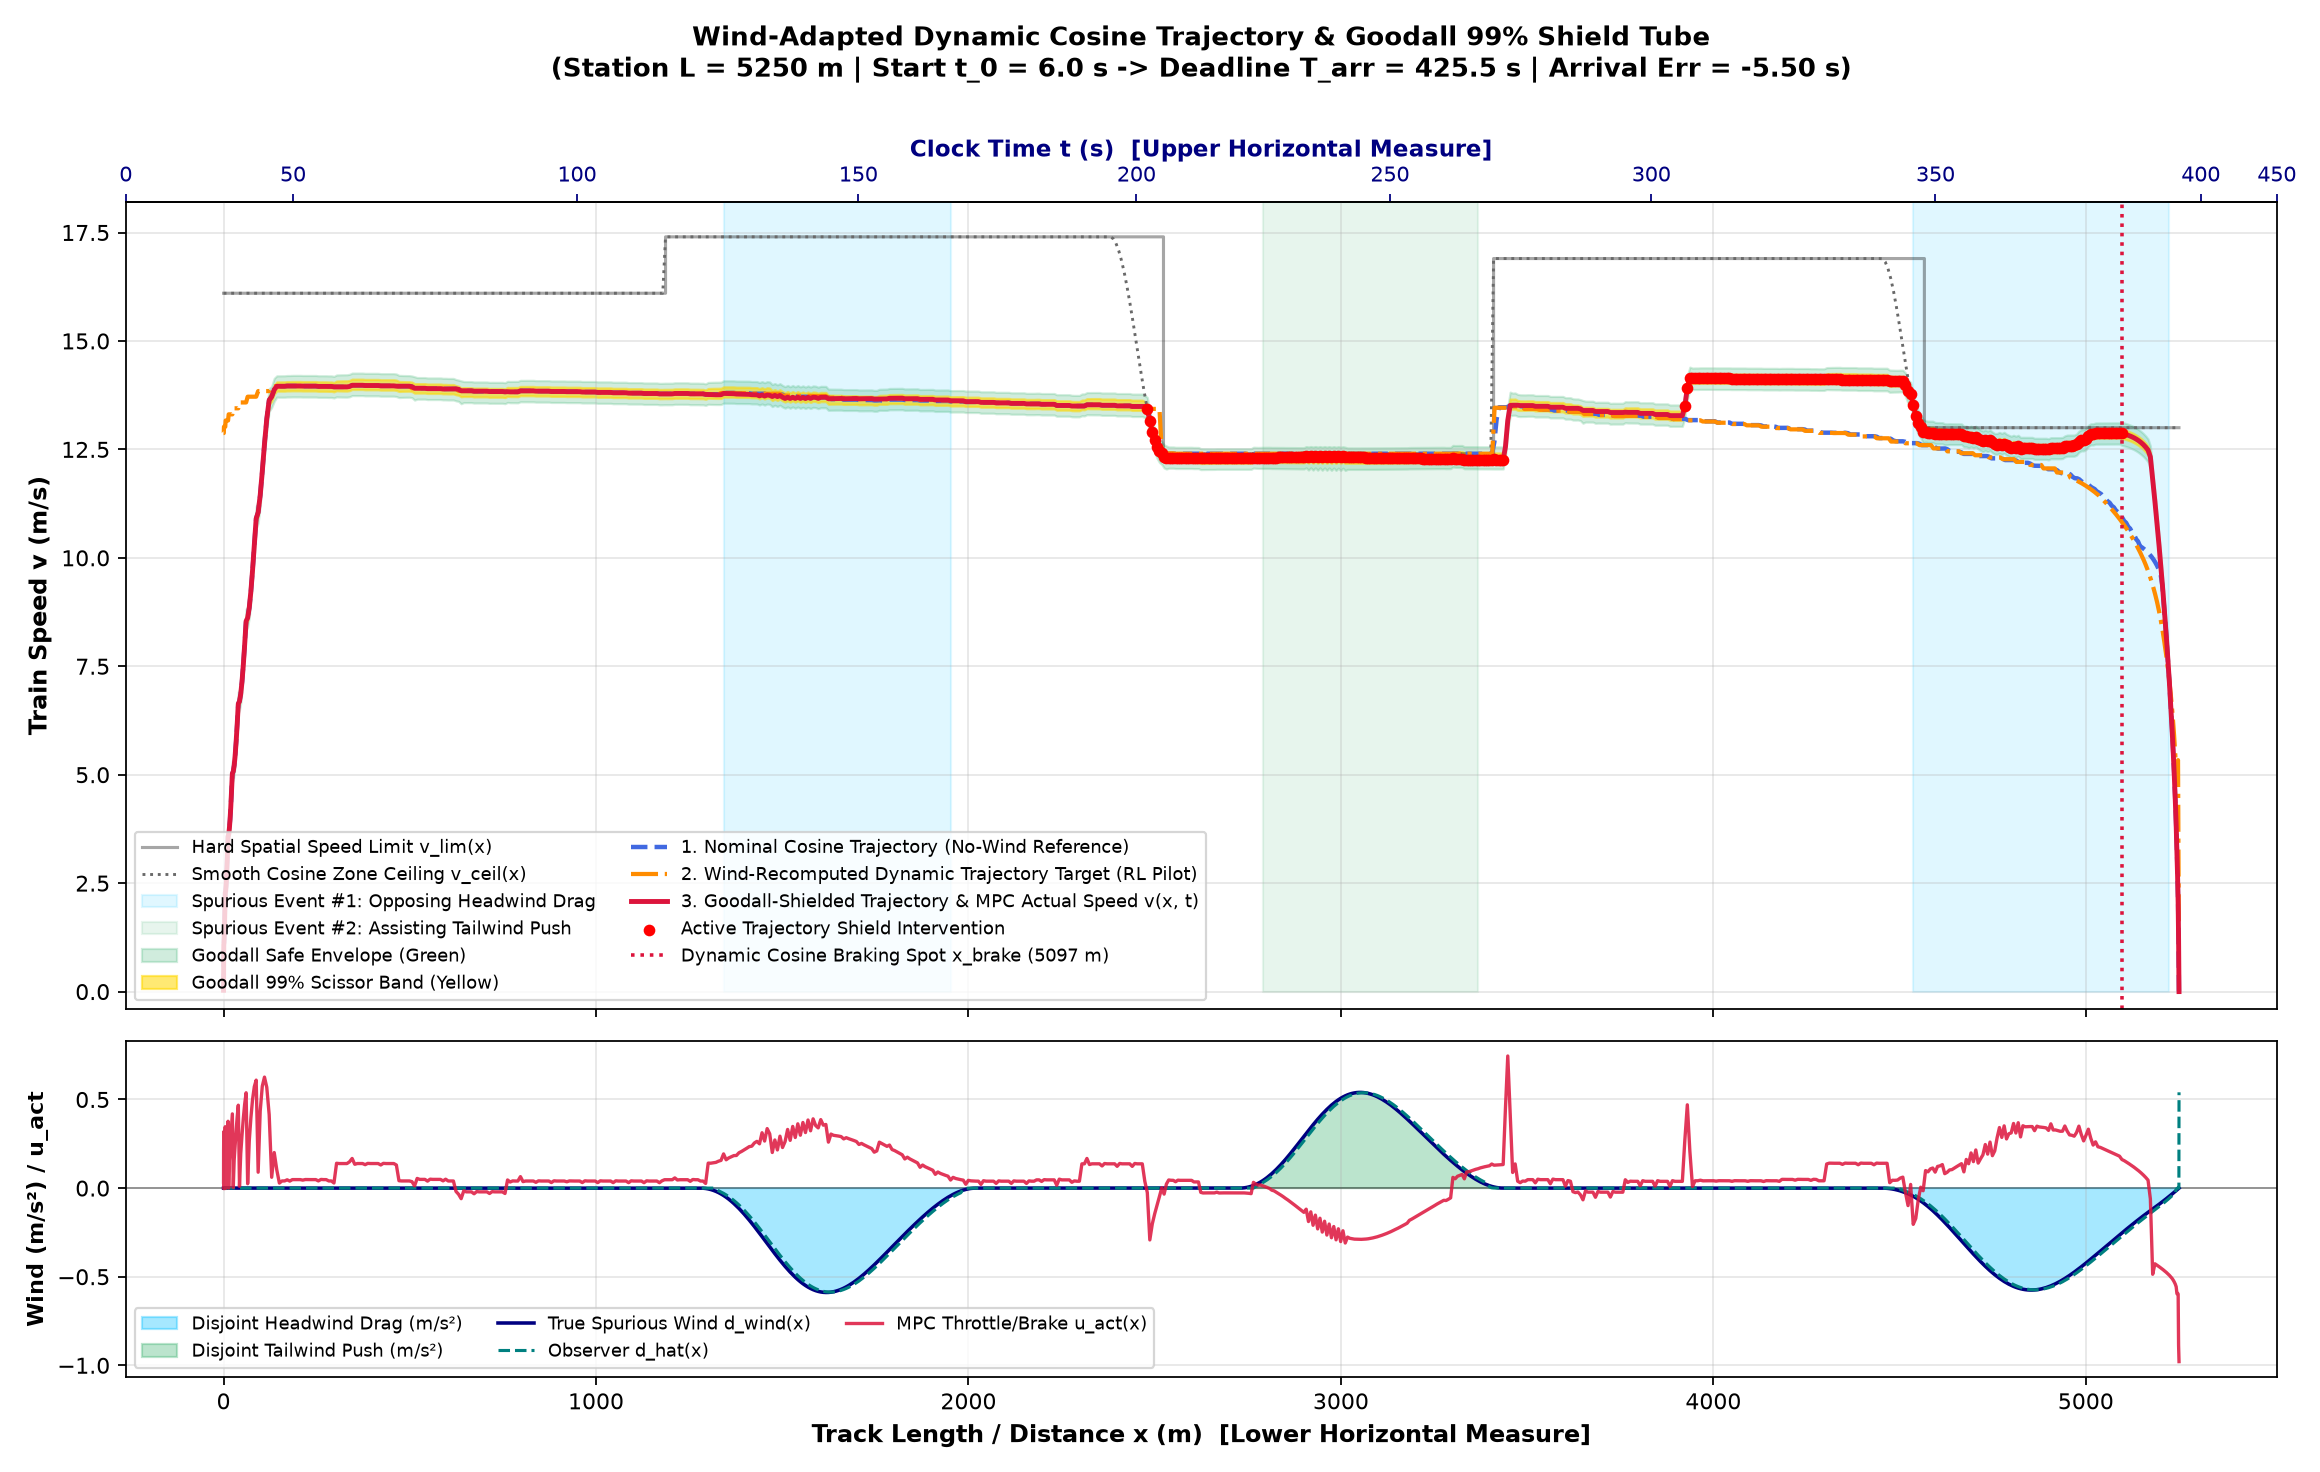
\includegraphics[width=0.98\textwidth]{wind_trajectory_shield_dual_axis.png}
\caption{Dual-horizontal-axis 4-station ($21.35\text{ km}$) evaluation showing cumulative track length $x$ (m) on the lower horizontal axis and clock time $t$ (s) on the upper horizontal axis. \textbf{Top:} Nominal no-wind trajectory (blue dashed), wind-recomputed PPO target (orange dash-dot), and Contract-Shielded MPC actual velocity (red solid) inside the Goodall 99\% Scissor Band (yellow) and Safe Envelope (green). \textbf{Bottom:} Headwind/tailwind events, MPC actuator effort $u_{\text{act}}$, and the 8-step concluded passenger mass $\hat{M}(x)$ converging onto the true train mass $M(x)$.}
\label{fig:dual_axis}
\end{figure}

\begin{figure}[h!]
\centering
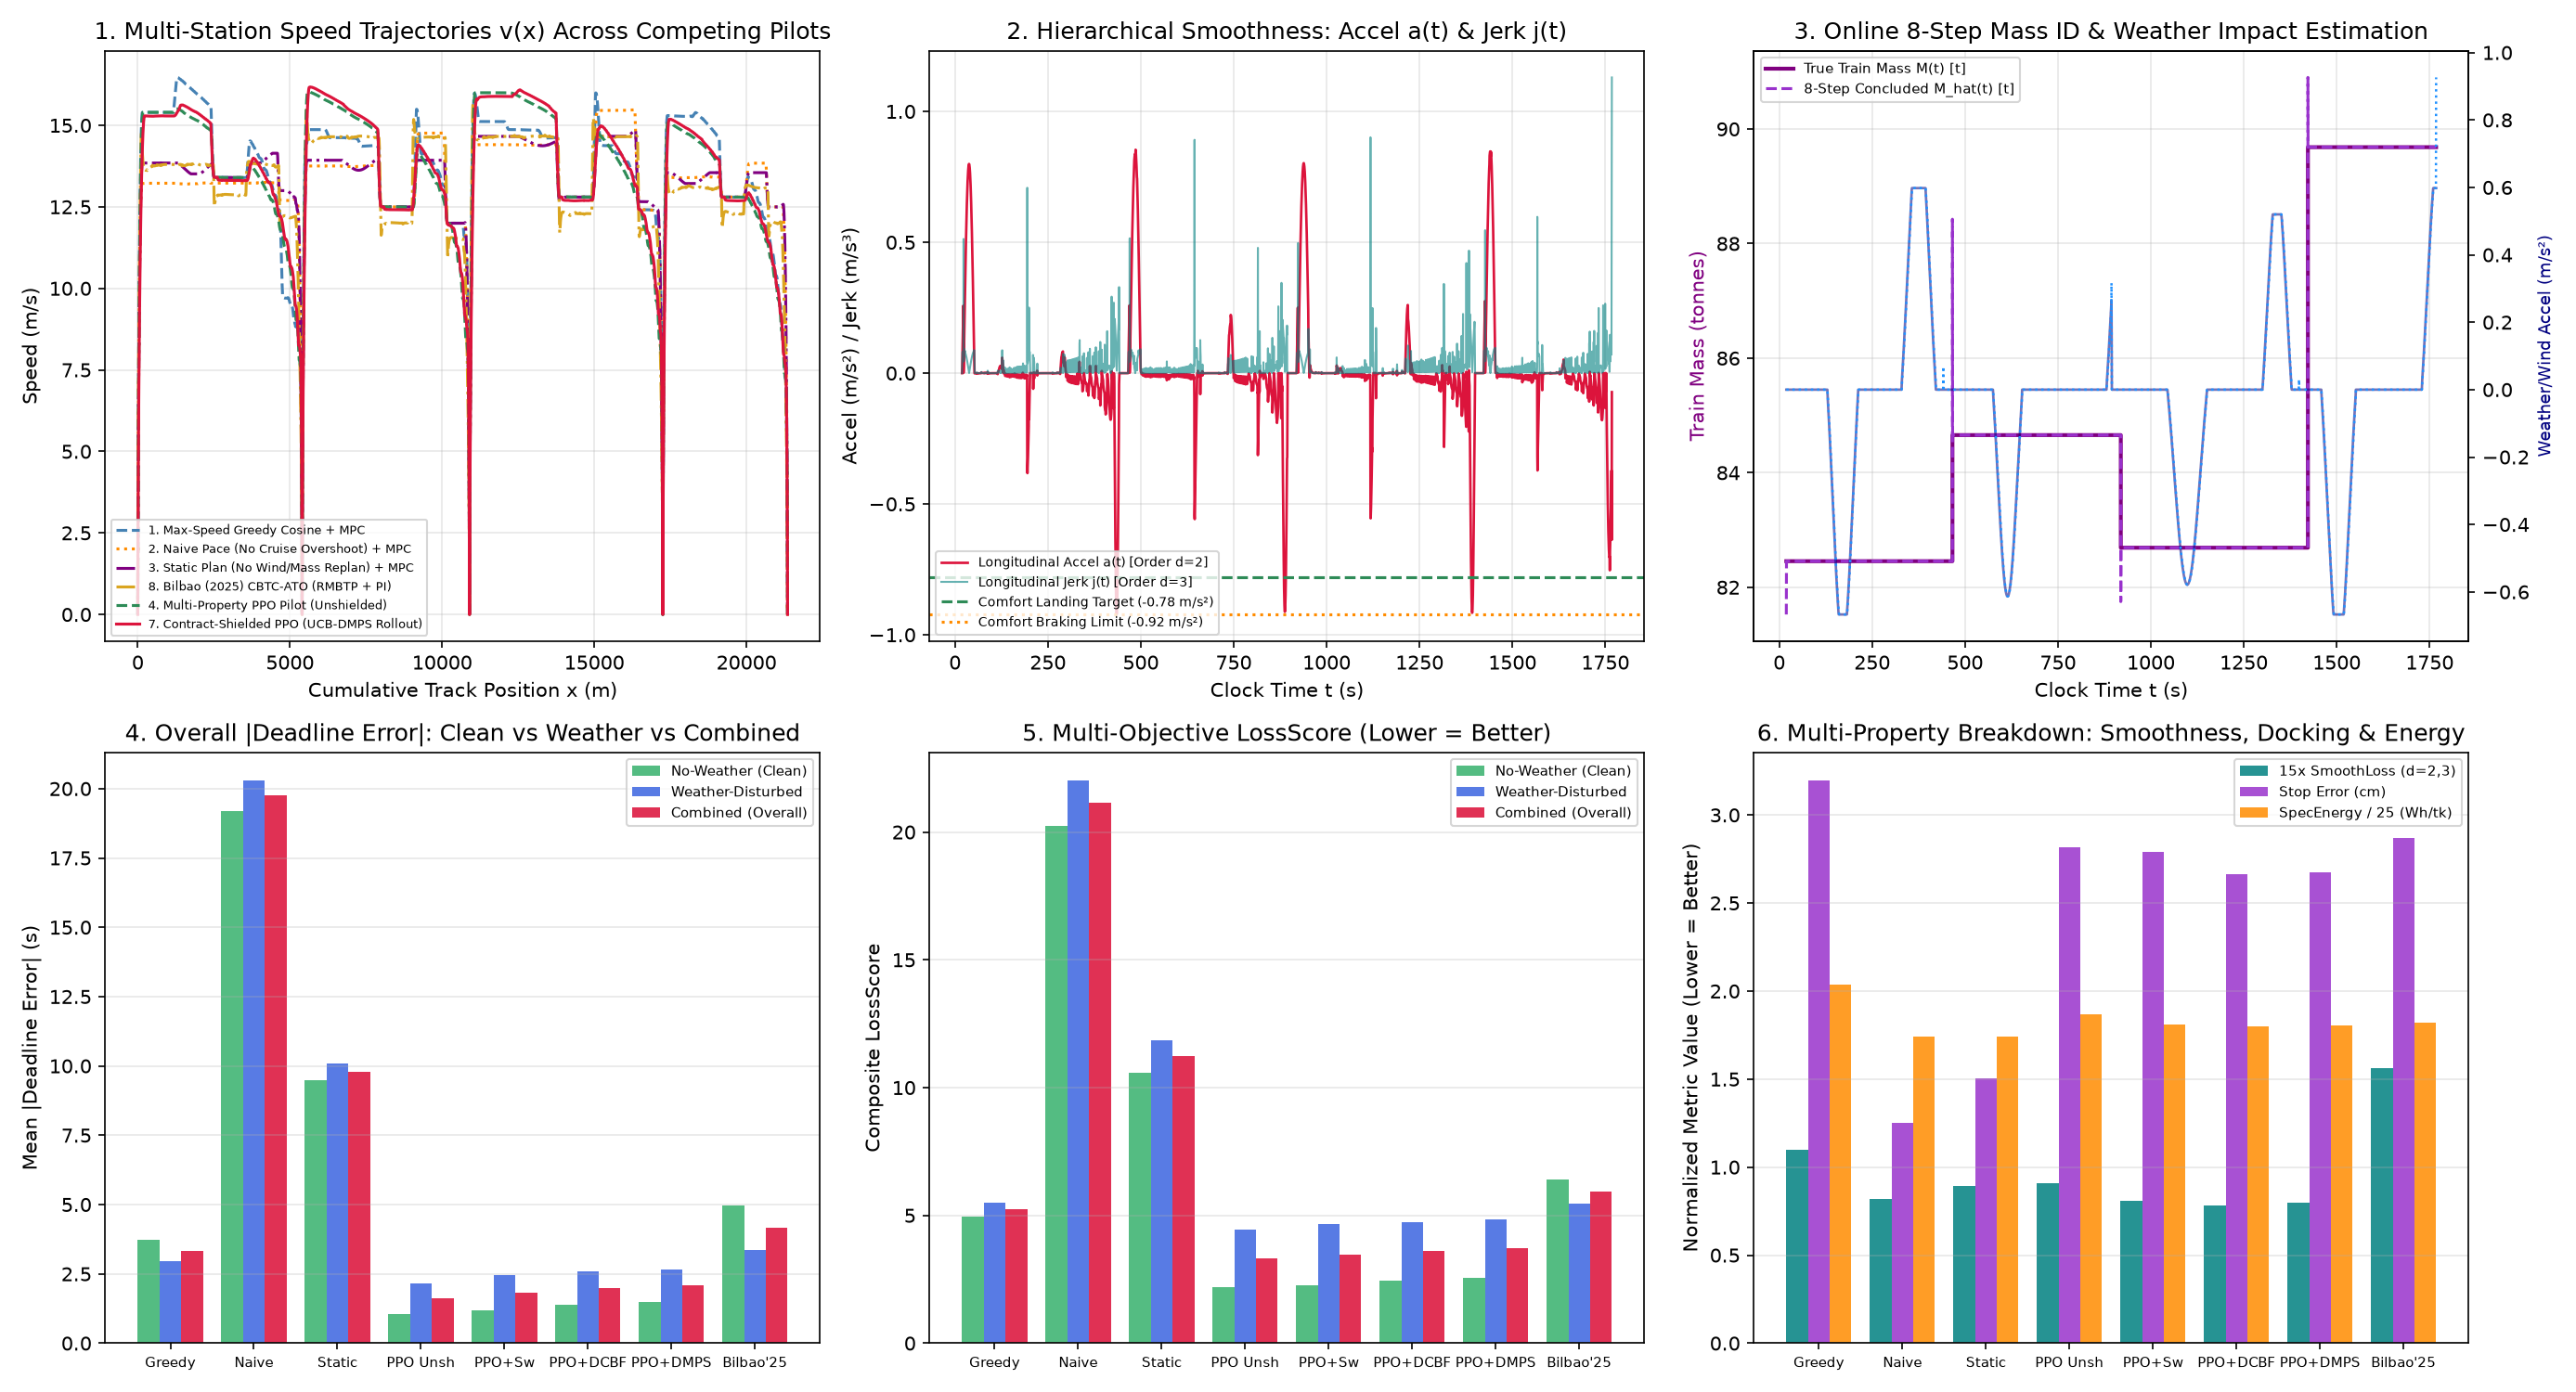
\includegraphics[width=0.98\textwidth]{rl_cosine_mpc.png}
\caption{Six-panel generalized benchmark overview across all 8 competing controllers: (1) multi-station speed profiles $v(x)$ including Bilbao et al.\ (2025) CBTC-ATO \cite{bilbao2025}, (2) smooth Order-2 acceleration $a(t)$ and Order-3 jerk $j(t)$, (3) online 8-step passenger mass identification and weather observer $\hat{d}(t)$, (4) mean deadline error across Clean, Weather-Disturbed, and Combined runs, (5) composite multi-objective LossScore, and (6) normalized breakdown of $15\times\text{SmoothLoss}$, Stop Error (cm), and $\text{SpecEnergy}/25$ (Wh/t-km).}
\label{fig:six_panel}
\end{figure}

\section{Discussion and Conclusions}

\begin{enumerate}[leftmargin=*]
    \item \textbf{Why Max-Speed Greedy Suffers in Smoothness and Energy:} When the Max-Speed Greedy baseline maximizes cruise speed with steep ramps ($a_{\text{start}} = 1.18\text{ m/s}^2$, $b_{\text{land}} = 0.90\text{ m/s}^2$) until ahead of schedule, its sharp acceleration and late braking drive up Order-2/3 smoothness loss ($\text{SmoothLoss} = 0.0733$) and inverter/friction energy losses ($50.86\text{ Wh/t-km}$), whereas our PPO pilot achieves more than $2\times$ better schedule accuracy ($1.61\text{ s}$ vs.\ $3.34\text{ s}$) at $4.2\text{ Wh/t-km}$ lower specific energy.
    \item \textbf{How Contract Latching Improves Both Ride Comfort and Energy:} By detecting the start of speed ramps and station departures and latching gentler backup contracts ($a_{\text{cap}} \approx 0.80\text{ m/s}^2$, $b_{\text{cap}} \approx 0.68\text{ m/s}^2$) for the ramp duration, the Contract Shield cuts $\text{SmoothLoss}$ by $13.7\%$ (from $0.0606$ to $0.0523$) and saves $1.74\text{ Wh/t-km}$ of traction energy while intervening on only $7.9\%\text{--}8.8\%$ of macro-steps.
    \item \textbf{Understanding Panel 6 (Normalized Multi-Property Breakdown):} Because raw $\text{SmoothLoss} \approx 0.05\text{--}0.10$, stopping error $\approx 0.028\text{ m}$, and specific energy $\approx 45\text{ Wh/t-km}$ span three different orders of magnitude, Panel 6 in Figure~\ref{fig:six_panel} plots $15 \times \text{SmoothLoss}$, $\text{Stop Error in cm}$ ($100 \times |\text{StopErr}|$), and $\text{SpecEnergy} / 25$ side by side on a shared $[0, 3.2]$ vertical axis so their physical trade-offs are directly visible.
    \item \textbf{Comparison with Bilbao-Moreno et al.\ (2025) CBTC-ATO \cite{bilbao2025}:} Implementing Bilbao-Moreno et al.'s RMBTP planner (with Regula Falsi ECO speed selection and backward braking curves) and Cascade PI controller (with the Braking Switcher) on our exact corridor problem reveals a clear trade-off. Their analytical zone planner and PI loops execute in just $21.2\text{ }\mu\text{s}$ per step and outperform Naive ($19.75\text{ s}$) and Static ($9.79\text{ s}$) baselines with a $4.15\text{ s}$ mean deadline error and $2.9\text{ cm}$ stopping error. However, because RMBTP plans constant-rate trapezoidal ramps ($90\%$ effort) rather than $C^2$ half-cosine S-curves, and because the Braking Switcher disconnects position feedback during deceleration, its smoothness loss is nearly twice as high as our Contract-Shielded PPO ($0.1041$ vs.\ $0.0523$) and its arrival error is $2\times$ larger ($4.15\text{ s}$ vs.\ $1.61\text{--}2.07\text{ s}$).
\end{enumerate}

\begin{thebibliography}{99}
\footnotesize
\bibitem{havaei2022} P. Havaei and M. A. Sandidzadeh, ``Intelligent-PID controller design for speed track in automatic train operation system with heuristic algorithms,'' \textit{Journal of Rail Transport Planning \& Management}, vol. 22, p. 100321, 2022.
\bibitem{liu2025} D. Liu, G. Yan, J. Zhou, and B. Chen, ``MPC-Based Speed Tracking Control for Subway Trains Under Actuator Constraints,'' \textit{Actuators}, vol. 14, no. 3, p. 134, 2025.
\bibitem{banerjee2024} A. Banerjee, K. Rahmani, J. Biswas, and I. Dillig, ``Dynamic Model Predictive Shielding for Provably Safe Reinforcement Learning,'' \textit{arXiv preprint arXiv:2405.13863}, 2024.
\bibitem{goodall2026} A. W. Goodall and F. Belardinelli, ``Safe Reinforcement Learning via Recovery-based Shielding with Gaussian Process Dynamics Models,'' in \textit{Proc. 25th Int. Conf. on Autonomous Agents and Multiagent Systems (AAMAS)}, 2026, pp. 540--549.
\bibitem{goodall_code} A. W. Goodall, ``A2C-GP-Shield: Official Implementation of Safe Reinforcement Learning via Recovery-based Shielding with Gaussian Process Dynamics Models,'' GitHub Repository, 2026.
\bibitem{hsu2024} K.-C. Hsu, H. Hu, and J. F. Fisac, ``The Safety Filter: A Unified View of Safety-Critical Control in Autonomous Systems,'' \textit{Annual Review of Control, Robotics, and Autonomous Systems}, vol. 7, pp. 47--72, 2024.
\bibitem{wang2023} Y. Wang et al., ``Enforcing Hard Constraints with Soft Barriers: Safe Reinforcement Learning in Unknown Stochastic Environments,'' in \textit{Proc. 40th Int. Conf. on Machine Learning (ICML)}, PMLR, vol. 202, 2023, pp. 36593--36604.
\bibitem{cannon2010} M. Cannon, B. Kouvaritakis, and X. Wu, ``Model predictive control for systems with stochastic disturbances and uncertain dynamics,'' \textit{Automatica}, vol. 46, no. 6, pp. 1195--1204, 2010.
\bibitem{mayne2005} D. Q. Mayne, M. M. Seron, and S. V. Rakovi\'{c}, ``Robust model predictive control of constrained linear systems with bounded disturbances,'' \textit{Automatica}, vol. 41, no. 2, pp. 219--224, 2005.
\bibitem{cano2026} F. Cano, T. A. Henzinger, and K. Kueffner, ``Shielding for Higher-Order Safety,'' \textit{arXiv preprint arXiv:2608.03662v1}, Aug. 2026.
\bibitem{adalat2026a} O. Adalat, E. Hamel-De le Court, and F. Belardinelli, ``Contract-Based Compositional Shielding for Safe Multi-Agent Reinforcement Learning,'' \textit{arXiv preprint arXiv:2606.14130v2}, Jul. 2026.
\bibitem{adalat2026b} O. Adalat, E. Hamel-De le Court, and F. Belardinelli, ``Contract-enabled Communication for Safe Multi-Agent Reinforcement Learning,'' in \textit{Proc. 26th Int. Conf. on Autonomous Agents and Multiagent Systems (AAMAS)}, 2027.
\bibitem{agarwal2021} A. Agarwal, S. M. Kakade, J. D. Lee, and G. Mahajan, ``On the Theory of Policy Gradient Methods: Optimality, Approximation, and Distribution Shift,'' \textit{Journal of Machine Learning Research (JMLR)}, vol. 22, no. 98, pp. 1--76, 2021.
\bibitem{mei2020} J. Mei, C. Xiao, C. Szepesv\'{a}ri, and D. Schuurmans, ``On the Global Convergence Rates of Softmax Policy Gradient Methods,'' in \textit{Proc. 37th Int. Conf. on Machine Learning (ICML)}, PMLR, vol. 119, 2020, pp. 6820--6829.
\bibitem{bilbao2025} A. Bilbao-Moreno, I. Elorza, E. Irigoyen, and I. Trojaola, ``ATO system for CBTC-based railways: Planning and disturbance estimation for enhanced automation,'' \textit{Results in Engineering}, vol. 26, p. 105357, 2025.
\end{thebibliography}

\end{document}
